\documentclass[journal]{IEEEtran}
\IEEEoverridecommandlockouts
\usepackage{cite}
\usepackage{amsmath,amssymb,amsfonts}
\usepackage{algorithmic}
\usepackage{algorithm}
\usepackage{graphicx}
\usepackage{textcomp}
\usepackage{xcolor}
\usepackage{booktabs}
\usepackage{amsmath}
\DeclareMathOperator*{\argmax}{arg\,max}
\usepackage{array}
\usepackage{hyperref}
\newtheorem{theorem}{Theorem}
\newtheorem{corollary}{Corollary}
\newtheorem{proposition}{Proposition}
\newtheorem{definition}{Definition}
\hypersetup{colorlinks=true, linkcolor=blue, citecolor=blue, urlcolor=blue}

\def\BibTeX{{\rm B\kern-.05em{\sc i\kern-.025em b}\kern-.08em
    T\kern-.1667em\lower.7ex\hbox{E}\kern-.125emX}}

%% Shorthand macros
\newcommand{\IL}{\mathcal{IL}}
\newcommand{\IO}{\mathcal{IO}}
\newcommand{\MGIL}{\mathcal{MGIL}}
\newcommand{\SGIO}{\mathcal{SGIO}}
\newcommand{\FO}{\mathcal{FO}}
\newcommand{\Faug}{\mathcal{F}_{\mathrm{aug}}}
\newcommand{\Fobs}{\mathcal{F}_{\mathrm{obs}}}
\newcommand{\Nb}{\mathcal{N}}
\newcommand{\bx}{\mathbf{x}}
\newcommand{\bz}{\mathbf{z}}
\newcommand{\btheta}{\boldsymbol{\theta}}
\newcommand{\blambda}{\boldsymbol{\lambda}}
\newcommand{\bW}{W_S}
\newcommand{\xbar}{\bar{\mathbf{x}}}
\newcommand{\R}{\mathbb{R}}
\newcommand{\cR}{\mathcal{R}}
\newcommand{\cP}{\mathcal{P}}
\newcommand{\cA}{\mathcal{A}}

\newcommand{\todo}[1]{\textcolor{red}{#1}}
\newcommand{\bX}{\mathbf{X}}
\newcommand{\zmean}{\bar{\mathbf{z}}}



\begin{document}

\title{Similarity-Guided Inverse Optimization for Personalized\\
Dietary Recommendations via Food Swapping}

\author{%
  Farzin~Ahmadi$^{1,2}$,
  Felix~Parker$^{2}$,
  Layne~C.~Price$^{3}$,
  Raviteja~Anantha$^{3}$,
  Valerie~K.~Sullivan$^{4,5}$,
  Lawrence~J.~Appel$^{4,5,6}$,
  and Kimia~Ghobadi$^{2}$%
  \thanks{$^{1}$Department of Health Sciences, Towson University, Towson, MD, USA.}%
  \thanks{$^{2}$Center for Systems Science and Engineering,
    Johns Hopkins University, Baltimore, MD 21218, USA.}%
  \thanks{$^{3}$Amazon.com, Seattle, WA, USA.}%
  \thanks{$^{4}$Welch Center for Prevention, Epidemiology, and Clinical Research, Johns Hopkins University, Baltimore, MD, USA}%
  \thanks{$^{5}$Department of Epidemiology, Bloomberg School of Public Health, Johns Hopkins University, Baltimore, MD, USA}%
  \thanks{$^{6}$Department of Medicine, Johns Hopkins School of Medicine, Baltimore, MD, USA}%
}

\maketitle

%% ============================================================
\begin{abstract}
%% ============================================================
Translating dietary guidelines into actionable, personalized food
recommendations remains a central challenge in nutrition informatics.
Existing approaches either operate at the abstract nutrient level, which
is clinically sound but not actionable, or rely on heuristic food
substitution rules that lack optimality guarantees. We propose
\textbf{Similarity-Guided Inverse Optimization (SGIO)}, a framework that
integrates a food item similarity matrix with the Inverse Optimization
(MGIL) optimization framework to produce item-level food swap
recommendations. Given a participant's observed dietary intake, we
augment the optimization decision space with the top-$K$ most similar
food items for each consumed food, encoding similarity scores as
switching costs in the inverse optimization objective. As DASH
nutritional constraints are progressively activated along the MGIL
tradeoff path, the model generates specific, ranked food swaps rather
than abstract group-level adjustments. We validate SGIO on 356 NHANES
2017--2018 participants using a Day~2 dietary recall holdout:
recommendations from Day~1 are benchmarked against the participant's own
unaided Day~2 eating behavior. SGIO recommendations at the first
tradeoff iteration ($r{=}1$) achieve a median normalized nutrient
distance of 1.991 from Day~1 intake, versus a natural intra-person
Day~1$\to$Day~2 median of 3.143 (Wilcoxon $W{=}11{,}055$,
$p{<}0.001$) --- a 37\% reduction. In food-item space, 84\% of $r{=}1$
recommendations fall below the cohort natural Day~2 median (median food
distance 238~g vs.\ natural 1,224~g; $p{<}0.001$). Recommendations
remain statistically within natural intra-person variance through
\emph{all four} constraint-tightening iterations ($p{<}0.001$ at each
$r \in \{1,2,3,4\}$ in both nutrient and food-item space), with only
3\% of participants classified as non-amenable. We further demonstrate
cross-dataset generalizability on 200 MyFitnessPal users via
temporal-split holdout validation, achieving a 47\% median nutrient
distance reduction ($W{=}153$, $p{<}0.001$) with 0\% non-amenable
rate, reflecting the broader substitution flexibility available in
multi-day food logs.
\end{abstract}

\begin{IEEEkeywords}
inverse optimization, dietary recommendations, food similarity,
personalized nutrition, DASH diet, NHANES, MyFitnessPal,
food swapping, multi-observation, temporal-split validation
\end{IEEEkeywords}

%% ============================================================
\section{Introduction}
\label{sec:intro}
%% ============================================================

Hypertension affects nearly half of U.S.\ adults and will develop in
approximately 4 in 5 Americans with advancing age~\cite{jones2025aha}.
It is a leading modifiable risk factor for cardiovascular disease and
stroke, making it one of the most prevalent and consequential chronic
conditions in the country. The Dietary Approaches to Stop Hypertension
(DASH) dietary pattern was specifically developed to address this risk,
and rigorously designed randomized controlled feeding trials have
demonstrated that adherence to a DASH diet produces clinically
meaningful reductions in blood
pressure~\cite{appel1997dash,sacks2001effects}. Yet population-level
adherence in the U.S.\ remains below
20\%~\cite{liese2009adherence}. Trials in free-living participants have
achieved sustained blood pressure reductions through intensive,
structured behavioral counseling to improve DASH
adherence~\cite{appel2003premier,blumenthal2010premier}; however,
the resource demands of such programs limit their widespread
implementation, motivating the development of lower-intensity,
scalable strategies to translate DASH targets into actionable,
personalized dietary guidance.

The core barrier to such strategies is a translation gap: nutritional
science operates in the language of nutrients, while human behavior
operates in the language of specific foods. Telling a patient to
``reduce sodium by 800~mg/day'' is clinically precise but practically
useless---few people eat nutrients, and no one shops for them. The
alternative---handing a patient a list of acceptable foods based on
generic dietary rules---ignores what they actually eat and is therefore
unlikely to stick.

This paper closes that gap with two interlocking contributions. The
first is a \emph{structured food similarity tool}: a multi-signal scoring
architecture (Section~\ref{sec:similarity}) combining dense embedding
retrieval over USDA FoodData Central~\cite{usda_2019}, macronutrient
profile matching, food category overlap, and LLM-based reranking, which
scores how substitutable any two foods are. Two foods with high
similarity are interchangeable both nutritionally and behaviorally. The
second is encoding those similarity scores directly as \emph{switching
costs} in a personalized optimization. When the optimizer is forced to
satisfy an additional DASH constraint, it pays a low cost to swap a
consumed food for a similar neighbor, and a high cost to substitute
something unfamiliar. Every recommended diet is \emph{guaranteed to be
fully DASH-feasible by construction}; the tradeoff path controls how
aggressively constraints are activated, not whether they hold.

We integrate the similarity matrix into the Modified Goal-Integrated
Inverse Learning ($\MGIL$) framework~\cite{ahmadi2024IL}, which
recovers an individual's latent dietary preferences from observed intake.
Prior formulations operated at the food group level, requiring a heuristic
post-processing step to translate group adjustments into specific swaps ---
a step that discards the optimization structure. Our formulation,
\textbf{SGIO} (Similarity-Guided Inverse Optimization), operates directly
at the food item level: each consumed food is paired with its top-$K$
most similar neighbors, and the optimizer selects swaps from this
personalized candidate set. A key open question for any such system is
behavioral realism: do recommendations require departures from habitual
behavior beyond what individuals naturally exhibit day-to-day? We address
this through holdout validation on 356 NHANES 2017--2018 participants,
using each individual's Day~2 dietary recall as a benchmark for natural
intra-person variation, and on 200 MyFitnessPal users via temporal-split
holdout.

The broader inverse optimization literature has developed methods for
learning from noisy observations~\cite{aswani2018inverse}, contextual
and online settings~\cite{besbes2023contextual}, uncertainty
quantification~\cite{lin2024conformal}, and improved loss functions and
algorithms~\cite{zattoni2025learning,elmachtoub2022smart}. IO has also
been applied in clinical settings such as cancer radiotherapy treatment
planning~\cite{chan2014generalized}, establishing a precedent for
learning patient-specific preference structures from clinical data;
SGIO extends this line of work to the dietary health domain.

Our contributions are:
\begin{enumerate}
\item A \textbf{multi-signal food similarity architecture} combining
dense embedding retrieval, macronutrient profile matching, food
category overlap, and LLM-based reranking, producing a
substitutability-informed similarity matrix over USDA FoodData Central
items and cross-database mappings to external food databases.
\item A \textbf{personalized augmented item space} that expands each
participant's observed intake with the top-$K$ most similar USDA food
items, derived from a precomputed similarity matrix.
\item A \textbf{similarity-discounted objective} encoding substitutability
as switching costs within the MGIL formulation, preserving all key
theoretical properties of the underlying framework.
\item An \textbf{item-level tradeoff path} in which each iteration
produces ranked, specific food swaps with quantified behavioral costs.
\item A \textbf{multi-dataset holdout validation} on 356 NHANES
participants (Day~2 recall) and 200 MyFitnessPal users (temporal-split
food logs), establishing that SGIO recommendations fall within natural
intra-person dietary variance across two distinct dietary data modalities.
\item A \textbf{multi-observation IO formulation} that, given
longitudinal daily intake data, produces per-day recommendations sharing
a common active constraint set, capturing constraints that are
consistently binding across an individual's eating pattern rather than
binding only on the average.
\end{enumerate}

%% ============================================================
\section{Background}
\label{sec:background}
%% ============================================================

The Inverse Optimization (IO) framework~\cite{ahmadi2024IL} addresses the
setting where a decision-maker's observed behavior
$\mathcal{X} = \{x^k\}_{k=1}^K$ is assumed to be noisy observations
of a latent optimal decision $z_0$ under an unknown objective $\theta$.
Given a known feasible set $\Omega$ (here, DASH nutritional constraints),
$\IL$ recovers $z_0$ by solving:
\begin{equation}
\IL(\mathcal{X},\Omega):\;\min_{z,\theta,\lambda}\;\sum_k\|x^k - z\|_2^2
\;\;\text{s.t. KKT}(z,\theta,\lambda,\Omega),
\label{eq:IL}
\end{equation}
where the KKT conditions enforce that $z$ is optimal for the forward
problem $\FO(\theta,\Omega)$. For squared Euclidean loss, the objective
reduces to $K\|z-\xbar\|_2^2$, making the formulation independent of
observation count $K$~\cite{ahmadi2024IL}.

Modified Goal-Integrated Inverse Learning ($\MGIL$) extends $\IO$ by
navigating the \emph{Observation-Constraint Tradeoff}: starting from the
unconstrained solution $z_0$, it iteratively forces additional DASH
constraints to bind while inheriting all previously active constraints.
This produces a sequence $\{z_\ell\}_{\ell=0}^L$ with monotonically
increasing distance to observations $D_\ell = \sum_k\|x^k-z_\ell\|_2^2$,
each $z_\ell$ lying on a nested face of $\Omega$~\cite{ahmadi2024IL}.
The marginal cost $\Delta D_\ell = D_{\ell+1} - D_\ell$ quantifies
the behavioral friction of satisfying one additional nutritional
constraint.

In prior work, decision variables $z$ represent servings of 38
\emph{food groups} derived from aggregating 5,000+ USDA items. This
aggregation enables tractability but sacrifices item-level specificity.

We further note that aggregating $K$ observations into their centroid,
while convenient, collapses all intra-person dietary variation into a
single average vector. For longitudinal data with $K \gg 2$ daily
observations, as available in food-logging platforms, a constraint that
appears tight on the centroid may not be tight on any individual day.
We address this limitation in Section~\ref{subsec:multi_obs}.

%% ============================================================
\section{Food Similarity Scoring}
\label{sec:similarity}
%% ============================================================

The food similarity matrix underlying SGIO requires a scoring
architecture that captures multiple facets of substitutability:
semantic identity (is this the same kind of food?), nutritional
proximity (do the two items have comparable macronutrient profiles?),
and categorical alignment (do they belong to the same food group?).
This section describes the representation, scoring components, matrix
construction, reranker refinement, and cross-database mapping
that together produce the similarity scores consumed by the SGIO
formulation.

\subsection{Food Item Representation}
\label{subsec:representation}

Each food item is represented as a structured text string combining its
name, brand, and food category tags:
\begin{quote}
\texttt{\{name\}. by \{brand\}. Categories: \{cat$_1$\}, \{cat$_2$\}, \ldots}
\end{quote}
The name field carries the primary product identity (e.g., ``Chocolate
Spread''). The brand field, when available, disambiguates products
sharing the same generic name; in practice, brand is a strong driver
of similarity scores for packaged and processed foods, where nutrient
profiles and serving conventions vary significantly across manufacturers.
Up to five USDA food category tags are appended, each cleaned by
stripping locale prefixes and replacing hyphens with spaces. This representation serves as input to both the
embedding model (Section~\ref{subsec:embedding}) and the reranker
(Section~\ref{subsec:reranker}).

\subsection{Dense Embedding}
\label{subsec:embedding}

Each food item's text representation is encoded into a 1024-dimensional
dense vector using Qwen3-Embedding-0.6B~\cite{zhang2025qwen3embedding},
an instruction-aware embedding model built on a decoder-only language
model. Unlike classical encoder-based models, the embedding is extracted
from the hidden state of the final layer at the end-of-sequence token,
after the full input has been processed through causal self-attention.
The model is instruction-aware: query inputs are prepended with a
task-specific instruction (``Given a food item name, retrieve similar
food products'') that steers the embedding space toward the retrieval
objective, while document texts are encoded without an instruction
prefix. This asymmetric encoding allows the same model to serve
different retrieval tasks by varying only the instruction. All embeddings
are L2-normalized, so the inner product equals cosine similarity:
\begin{equation}
S_{ij}^{\mathrm{emb}} = \mathbf{e}_i^\top \mathbf{e}_j, \quad
\|\mathbf{e}_i\|_2 = 1 \;\;\forall\, i.
\label{eq:emb_sim}
\end{equation}
Normalized embeddings are indexed in a FAISS~\cite{johnson2019faiss}
flat inner-product index for exact nearest-neighbor retrieval.

\subsection{Macronutrient Profile Scoring}
\label{subsec:macro_scoring}

Embedding similarity captures semantic and behavioral similarity but
may not reflect explicit nutritional proximity. We complement it with
a macronutrient profile score computed over eight nutrient fields:
energy (kcal), fat, carbohydrates, protein, sugars, fiber, sodium, and
saturated fat, all measured per 100\,g.

For each nutrient $n$ where both items $i$ and $j$ have valid values,
we compute a logistic-transformed scaled L1 distance:
\begin{equation}
S_{ij}^{\mathrm{macro}} = \frac{1}{|N_{ij}|}\sum_{n \in N_{ij}}
\frac{1}{1 + |m_i^n - m_j^n| \,/\, s_n},
\label{eq:macro_sim}
\end{equation}
where $N_{ij}$ is the set of nutrients with valid values for both items,
$m_i^n$ is the value of nutrient $n$ for item $i$, and $s_n$ is an
IQR-based scale factor for nutrient $n$ derived from the source database
distribution. Nutrients missing for either item are excluded from the
pairwise average; pairs sharing no valid nutrients receive a score of~0.

\subsection{Category Scoring}
\label{subsec:category_scoring}

To encourage substitutions within the same food group, we compute the
Jaccard similarity over USDA food category tag sets:
\begin{equation}
S_{ij}^{\mathrm{cat}} =
\frac{|C_i \cap C_j|}{|C_i \cup C_j|},
\label{eq:cat_sim}
\end{equation}
where $C_i$ denotes the set of category tags assigned to item $i$.
Items with no category tags receive a score of~0 with all other items.

\subsection{Intra-Database Similarity Matrix}
\label{subsec:matrix}

The similarity matrix covers USDA FoodData Central items drawn primarily
from the FNDDS (Food and Nutrient Database for Dietary Studies)
2021--2023 taxonomy, the standard reference for NHANES dietary analysis,
supplemented by Foundation Foods entries where available. For these
7,338 items, we construct a full $N \times N$ pairwise similarity matrix
as a convex combination of the three component scores:
\begin{equation}
S_{ij}^{\mathrm{mat}} =
w_{\mathrm{emb}}\, S_{ij}^{\mathrm{emb}}
+ w_{\mathrm{macro}}\, S_{ij}^{\mathrm{macro}}
+ w_{\mathrm{cat}}\, S_{ij}^{\mathrm{cat}},
\label{eq:matrix_sim}
\end{equation}
with $w_{\mathrm{emb}} + w_{\mathrm{macro}} + w_{\mathrm{cat}} = 1$.
Default weights are $w_{\mathrm{emb}} = 0.56$, $w_{\mathrm{macro}} =
0.28$, and $w_{\mathrm{cat}} = 0.16$, reflecting the relative
informativeness of each signal: dense embeddings encode broad semantic
and behavioral substitutability (the primary signal), macronutrient
profiles provide direct nutritional grounding (a complementary but
narrower signal), and category tags encode coarser food-group alignment
(a regularizing signal). Since each component score lies in $[0,1]$,
the combined score $S_{ij}^{\mathrm{mat}} \in [0,1]$. We note that
equal weights ($w_{\mathrm{emb}} = w_{\mathrm{macro}} =
w_{\mathrm{cat}} = 1/3$) are also a reasonable choice; an ablation
comparing weighting schemes is identified as a future direction in
Section~\ref{sec:discussion}.

\subsection{LLM Reranker Refinement}
\label{subsec:reranker}

The embedding model encodes each item independently and scores via a dot
product, which is efficient for $N \times N$ computation but limited in
expressiveness. For refinement we apply
Qwen3-Reranker-0.6B~\cite{zhang2025qwen3embedding}, a pointwise
reranker built on the same decoder-only architecture as the embedding
model. The reranker jointly processes both items through causal
self-attention over a single concatenated sequence, yielding a more
precise substitutability judgment at the cost of quadratic inference. We
apply it only to the top-$K$ neighbors from the matrix.

The reranker frames relevance as a binary classification task within the
language model's chat template: given an instruction, a query (food item
name), and a document (candidate text), the model is prompted to judge
whether the document is relevant to the query. The relevance score is
the normalized likelihood of the ``yes'' token:
\begin{equation}
S_{ij}^{\mathrm{rr}} = \frac{e^{\,p(\text{yes} \mid f_i, f_j)}}
{e^{\,p(\text{yes} \mid f_i, f_j)} + e^{\,p(\text{no} \mid f_i, f_j)}},
\label{eq:reranker_sim}
\end{equation}
where $p(\cdot \mid f_i, f_j)$ denotes the next-token log-probability
at the final position of the prompt. The final refined similarity for
each top-$K$ neighbor is a convex combination of the matrix score and
reranker score:
\begin{equation}
S_{ij} =
w_{\mathrm{mat}}\, S_{ij}^{\mathrm{mat}}
+ w_{\mathrm{rr}}\, S_{ij}^{\mathrm{rr}},
\label{eq:refined_sim}
\end{equation}
with $w_{\mathrm{mat}} + w_{\mathrm{rr}} = 1$, default
$w_{\mathrm{mat}} = 0.5$, $w_{\mathrm{rr}} = 0.5$. The reranker
score receives equal weight to the matrix score, as it corrects
purely semantic retrieval errors at the cost of higher inference time.

\subsection{Cross-Database Food Mapping}
\label{subsec:mapping}

SGIO operates on USDA nutrient data, but dietary intake may be recorded
in external databases (e.g., MyFitnessPal food logs) whose items do not
appear in the USDA catalog. To bridge this gap, we map every item in a
source database to its $K$ nearest USDA neighbors via a two-stage
pipeline:
\begin{enumerate}
\item Embedding retrieval: cosine similarity between source and target
  embeddings selects $2K$ candidate USDA items per source item.
\item LLM reranking: all $2K$ candidates are re-scored by the
  reranker, and the top $K$ are retained.
\end{enumerate}
The final mapping score combines embedding and reranker scores using the
same weighted-average form as~\eqref{eq:refined_sim}. Target embeddings
are held in memory while source embeddings are streamed in batches,
keeping peak memory usage proportional to the target database size.

This mapping enables SGIO on non-USDA datasets: source food items are
bridged to USDA nutrient data via their nearest USDA neighbors,
providing both the nutrient matrix columns and the similarity scores
required by the augmented item space (Section~\ref{subsec:augspace}).
For the SGIO switching costs, we use the reranker score
$S_{ij}^{\mathrm{rr}}$ exclusively, as it provides the more
semantically precise substitutability signal. Cross-database mapping
accuracy has not been formally evaluated against a labeled ground truth;
mapping quality is an important direction for future validation,
particularly for foods with ambiguous names or high brand diversity.

\subsection{Manual Evaluation of Similarity Scores}
\label{subsec:sim_eval}

To assess whether the similarity scores reflect human judgments of food
substitutability, a nutrition researcher evaluated 214 food pairs drawn
from the FNDDS 2017--2018 database (7,338 items) via a web-based
interface that displayed both foods' names, macronutrient profiles, and
category tags but not the system's similarity scores. Two complementary
tasks were administered.

In the binary substitution task (107 pairs), the rater judged whether a
candidate drawn from the query food's top-5 neighbors would be a
reasonable meal-level replacement. The overall acceptance rate was
87.9\%. A clear threshold effect emerged at a similarity score of 0.50:
pairs scoring above this threshold were accepted at a 96\% rate, while
those below were accepted at only 69\%. Among pairs with scores above
0.80, the acceptance rate was 100\%. All 13 rejected pairs shared the
same WWEIA food category as their query (category Jaccard~$= 1.0$),
indicating that the primary failure mode is within-category variation in
preparation or form (e.g., sun-dried vs.\ cooked tomatoes, turkey
nuggets vs.\ canned turkey) rather than cross-category retrieval errors.

In the Likert similarity task (107 pairs), pairs were stratified across
five similarity bins, from bin~1 (different food groups, not neighbors)
to bin~5 (top-2 neighbors), and the rater assigned a 1--5 similarity
rating. Mean human ratings increased monotonically with the system's
similarity bin (1.00, 1.91, 3.67, 4.08, 4.58 for bins 1--5), yielding
a Spearman rank correlation of $\rho = 0.794$ ($p < 0.001$). Strong
discordance (system and rater fully disagree) occurred in only 3.7\% of
pairs. The rating distribution was bimodal, with 59\% of ratings at the
extremes (1 or 5), suggesting confident, decisive judgments that lend
credibility to the evaluation signal.

These results provide preliminary evidence that the multi-signal
similarity architecture produces scores that align well with human
substitutability judgments. A formal multi-rater validation with
inter-rater reliability analysis is identified as a future direction.


%% ============================================================
\section{Similarity-Guided Inverse Optimization (SGIO)}
\label{sec:smgil}
%% ============================================================

\subsection{Personalized Augmented Item Space}
\label{subsec:augspace}

Let participant $p$ have a recorded Day~1 intake consisting of $M$
distinct food items $\Fobs = \{f_1,\ldots,f_M\}$ with observed
quantities $\hat{x}_{f_i} > 0$. For each consumed item $f_i$, we retrieve its top-$K$ most similar
neighbors from the USDA catalog by reranker score
(Section~\ref{subsec:reranker}) --- in essence, a $k$-nearest-neighbor
lookup over the precomputed similarity matrix excluding already-consumed
foods:
\begin{equation}
\Nb_K(f_i) = \argmax_{\substack{j:\, j \neq f_i,\\ j \notin \Fobs}}
\{S_{f_i j} : j = 1,\ldots,|\mathcal{F}|\}_K.
\label{eq:neighbors}
\end{equation}
The \textbf{augmented item space} is:
\begin{equation}
\Faug = \Fobs \cup \bigcup_{i=1}^M \Nb_K(f_i),
\quad |\Faug| \leq M(1+K).
\label{eq:augspace}
\end{equation}

The observation vector $x^k \in \R^{|\Faug|}$ has $x^k_{f_i} =
\hat{x}_{f_i}$ for observed items and $x^k_j = 0$ for all neighbor
items $j \in \Nb_K(f_i)$. The nutrient matrix $A \in \R^{C \times
|\Faug|}$ is constructed directly from USDA FoodData Central at the
item level, with each column encoding the exact nutrient content per
gram of the corresponding food item, eliminating the group-averaging
approximation of prior work.

\subsection{Similarity-Discounted Objective}
\label{subsec:objective}

Define the weight diagonal matrix $\bW \in \R^{|\Faug| \times |\Faug|}$
by:
\begin{equation}
(\bW)_{jj} =
\begin{cases}
1 & \text{if } j \in \Fobs, \\
1 - S_{f_i(j),\, j} & \text{if } j \in \Nb_K(f_i),
\end{cases}
\label{eq:weights}
\end{equation}
where $f_i(j)$ denotes the consumed item whose neighbor set contains
$j$. When $S_{f_i(j),j} \approx 1$ (near-perfect substitute), the
penalty weight approaches zero, and the optimizer can freely substitute.
When $S_{f_i(j),j} \approx 0$, the weight equals 1, identical to the
penalty for reducing the consumed item itself.

\begin{proposition}[Positive Definiteness of $\bW$]
\label{prop:WSpd}
Under the condition that $S_{f_i(j),j} < 1$ for all neighbor items $j$,
$\bW \succ 0$.
\end{proposition}

Since $\bW \succ 0$, the weighted objective $\|z - \xbar\|_{\bW}^2 =
(z-\xbar)^\top \bW (z-\xbar)$ is strictly convex in $z$, preserving
unique solution identifiability. The centroid aggregation property
extends to the weighted case:
\begin{equation}
\sum_k \|x^k - z\|_{\bW}^2 = K\|z - \xbar\|_{\bW}^2 + \text{const},
\label{eq:aggregation}
\end{equation}
so the formulation remains independent of $K$ and admits streaming
updates $\xbar_{K+1} = \frac{K}{K+1}\xbar_K +
\frac{1}{K+1}x^{K+1}$.

\subsection{The SGIO Formulation}
\label{subsec:smgil_formulation}

Given observations $\mathcal{X}$, augmented item space $\Faug$, DASH
constraint set $\Omega = \{z \in \R^{|\Faug|}_+ : Az \leq b\}$,
constraint hierarchy $(\cR, \cP)$, seed solution $z_{\mathrm{prev}}$
with active set $\cA_{\mathrm{prev}}$, the SGIO formulation at
iteration $\ell$ is:

\begin{subequations}\label{eq:SMGIL}
\begin{align}
\SGIO:\;\min_{z,\btheta,\blambda,v}\;\;
& \omega \| z - \xbar \|_{\bW}^2
- (1-\omega)\sum_{i \in \cP} v_i
\label{eq:SMGIL-obj}\\
\text{s.t.}\;\;
& Az \leq b,\;\; z \geq 0,
\label{eq:SMGIL-feas}\\
& \btheta = A^\top \blambda,
\label{eq:SMGIL-stat}\\
& \btheta^\top z = b^\top \blambda,
\label{eq:SMGIL-sd}\\
& g_i(z) = 0,\;\; \forall i \in \cA_{\mathrm{prev}},
\label{eq:SMGIL-inherit}\\
& \blambda_i \leq M v_i,\;\; \forall i,
\label{eq:SMGIL-comp}\\
& g_i(z) \leq -\varepsilon(1-v_i),\;\;
  \forall i \in \cR\setminus\cA_{\mathrm{prev}},
\label{eq:SMGIL-slack}\\
& \sum_{i \in \cR\setminus\cA_{\mathrm{prev}}} v_i \geq 1,
\label{eq:SMGIL-increment}\\
& v_i \in \{0,1\},\;\blambda \geq 0,\;\btheta \in \Theta.
\label{eq:SMGIL-domain}
\end{align}
\end{subequations}

The formulation inherits the complete KKT structure of
$\MGIL$~\cite{ahmadi2024IL}: stationarity~\eqref{eq:SMGIL-stat} and
strong duality~\eqref{eq:SMGIL-sd} together with primal
feasibility~\eqref{eq:SMGIL-feas} and dual
feasibility~\eqref{eq:SMGIL-domain} ensure that any feasible $z$ is
forward-optimal for some $\btheta \in \Theta$.
Constraint~\eqref{eq:SMGIL-inherit} enforces inheritance of previously
active constraints, and~\eqref{eq:SMGIL-increment} forces at least one
new constraint to bind at each iteration.

\begin{corollary}[Inherited Theoretical Guarantees]
\label{thm:inherited}
The $\SGIO$ formulation \eqref{eq:SMGIL} inherits the following
properties directly from $\MGIL$~\cite{ahmadi2024IL}:
\begin{enumerate}
\item[(i)] \textbf{Complexity.} $O(|\Faug| + m)$ continuous variables,
$m$ binary variables, $O(|\Faug| + m)$ constraints, independent of $K$.
\item[(ii)] \textbf{Monotone distance.}
$D^{\bW}_0 \leq D^{\bW}_1 \leq \cdots \leq D^{\bW}_L$ where
$D^{\bW}_\ell = \|z_\ell - \xbar\|_{{\bW}}^2$.
\item[(iii)] \textbf{Face containment.}
$\cA_0 \subseteq \cA_1 \subseteq \cdots \subseteq \cA_L$, and each
$z_\ell$ lies on the face $\mathcal{F}_\ell \supseteq \mathcal{F}_{l+1}$.
\item[(iv)] \textbf{Forward optimality.} Each $z_\ell$ is optimal for
$\FO(\btheta_\ell, \Omega)$ under Slater's condition.
\end{enumerate}
\end{corollary}

\subsection{Item-Level Swap Extraction}
\label{subsec:swaps}

At each iteration $\ell$, the $\SGIO$ solution $z_\ell$ is a full
item-level quantity allocation. Food swaps are extracted by comparing
$z_\ell$ to the observed intake $\hat{x}$:

\begin{definition}[Food Swap at iteration $\ell$]
A \textbf{reduction} is $(f_i, \delta^-)$ with $\delta^- =
\hat{x}_{f_i} - (z_\ell)_{f_i} > 0$. A \textbf{substitution} is
$(f_i, j, \delta^+)$ with $j \in \Nb_K(f_i)$ and
$\delta^+ = (z_\ell)_j > 0$.
\end{definition}

Substitutions are ranked by similarity score $S_{f_i, j}$ within each
parent item's neighbor set. The marginal cost $\Delta D^{\bW}_\ell$
provides the behavioral price tag of the entire swap set at iteration
$\ell$, and serves as a natural stopping criterion: we halt when
$\Delta D^{\bW}_\ell > \tau$ for a user-specified threshold $\tau$.

\begin{algorithm}[t]
\caption{Similarity-Guided Inverse Optimization (SGIO)}
\label{alg:SMGIL}
\begin{algorithmic}[1]
\REQUIRE Intake $\hat{x}$, similarity matrix $S$, DASH
constraints $(\Omega, \cR, \cP)$, neighbors $K$, max iterations
$L_{\max}$, weight $\omega$, threshold $\tau$
\ENSURE Tradeoff path
$\{z_\ell, \btheta_\ell, D^{\bW}_\ell, \text{Swaps}_\ell\}_{\ell=0}^L$
\STATE Construct $\Faug$ via \eqref{eq:neighbors}--\eqref{eq:augspace}
\STATE Build $A$ from USDA FoodData Central for items in $\Faug$
\STATE Compute $\bW$ via \eqref{eq:weights}; compute $\xbar$
\STATE Solve $\IL(\{\hat{x}\}, \Omega)$ with objective
       $\|z-\xbar\|_{\bW}^2$ to obtain $z_0, \btheta_0$
\STATE $\cA_0 \leftarrow \{i \in \cR : g_i(z_0)=0\}$;\quad
       $D^{\bW}_0 \leftarrow \|z_0-\xbar\|_{\bW}^2$;\quad $\ell \leftarrow 0$
\WHILE{$\ell < L_{\max}$ \AND $|\cA_\ell| < |\cR|$}
    \STATE Solve $\SGIO$ \eqref{eq:SMGIL} to obtain $(z_{\ell+1},\btheta_{\ell+1})$
    \STATE $\Delta D^{\bW}_{\ell+1} \leftarrow
           \|z_{\ell+1}-\xbar\|_{\bW}^2 - D^{\bW}_\ell$
    \IF{$\Delta D^{\bW}_{\ell+1} > \tau$}
        \STATE \textbf{break}
    \ENDIF
    \STATE $\cA_{\ell+1}$, $D^{\bW}_{\ell+1}$, $\text{Swaps}_{\ell+1}$
           $\leftarrow$ update
    \STATE $\ell \leftarrow \ell + 1$
\ENDWHILE
\RETURN $\{z_\ell, \btheta_\ell, D^{\bW}_\ell, \text{Swaps}_\ell\}_{\ell=0}^L$
\end{algorithmic}
\end{algorithm}

\subsection{Multi-Observation Formulation}
\label{subsec:multi_obs}

The single-observation formulation aggregates $K$ observations into their
centroid $\xbar$ and produces a single allocation $z$. When $K$ daily
observations are available, as with multi-day food logs, this centroid
reduction discards information about day-to-day dietary variation. A
constraint that appears tight on the average $\xbar$ may not be tight on
any individual day; conversely, a constraint that is binding on every
observed day is a stronger signal of the individual's habitual dietary
limitation.

The multi-observation SGIO formulation introduces $K$ separate allocation
vectors $z_1, \ldots, z_K$, one per observed day, while sharing a single
set of binary constraint-selection variables $v$:
\begin{subequations}\label{eq:SMGIL-multi}
\begin{align}
\SGIO\text{-MO}:\;\min_{z_1,\ldots,z_K,\btheta,\blambda,v}\;\;
& \frac{1}{K}\sum_{k=1}^K \| x^k - z_k \|_{\bW}^2
\label{eq:multi-obj}\\
\text{s.t.}\;\;
& A z_k \leq b,\;\; z_k \geq 0,\;\; \forall k,
\label{eq:multi-feas}\\
& g_i(z_k) = 0,\;\; \forall k,\;\forall i \in \cA_{\mathrm{prev}},
\label{eq:multi-inherit}\\
& \blambda^k_i \leq M v_i,\;\; \forall k,\;\forall i,
\label{eq:multi-comp}\\
& g_i(z_k) \leq -\varepsilon(1-v_i),\;\;\\ &
  \forall k,\;\forall i \in \cR\setminus\cA_{\mathrm{prev}},
\label{eq:multi-slack}\\
& \sum_{i \in \cR\setminus\cA_{\mathrm{prev}}} v_i \geq 1,
\label{eq:multi-increment}\\
& v_i \in \{0,1\},\;\blambda^k \geq 0,\;\btheta \in \Theta.
\label{eq:multi-domain}
\end{align}
\end{subequations}

The key structural property is that the binary variables $v$ are
\emph{shared} across all $K$ days: when $v_i = 1$, constraint $i$ must
be tight for \emph{every} observation day simultaneously. The $1/K$
normalization in the objective makes the weighted distance comparable to
the single-observation case. The formulation has $O(Kn + m)$ continuous
variables, $m$ binary variables (unchanged from single-observation), and
$O(K(n + m))$ constraints, i.e., linear growth in $K$ for the continuous
part, with the combinatorial complexity (which dominates solve time in
MIQP) unchanged.

When $K = 1$, the multi-observation formulation reduces exactly to the
single-observation formulation~\eqref{eq:SMGIL}. All theoretical
guarantees of Corollary~\ref{thm:inherited} (monotone distance, face
containment, and forward optimality) carry over, since each $z_k$
individually satisfies the KKT conditions under the shared $\btheta$.
The mean recommendation $\zmean = \frac{1}{K}\sum_k z_k$ serves as the
consensus allocation for swap extraction.

%% ============================================================
\section{Experimental Evaluation}
\label{sec:experiments}
%% ============================================================

\subsection{Datasets and Setup}
\label{subsec:setup}

We evaluate SGIO on two dietary datasets spanning distinct data
collection modalities: interviewer-administered 24-hour recall (NHANES)
and self-reported food logs (MyFitnessPal). NHANES serves as the primary
evaluation; MFP demonstrates cross-modality generalizability.

\subsubsection{NHANES 2017--2018 (Primary)}
\label{subsubsec:nhanes_setup}

We use the NHANES 2017--2018 dietary recall
dataset~\cite{CDC_2020}. The analysis is restricted to adults
aged 18--75 years with complete dietary recall data, defined by the
interviewer-assessed data quality indicators DR1DRSTZ\,$= 1$ and
DR2DRSTZ\,$= 1$ for Day~1 and Day~2 respectively; these indicators flag
records as complete and usable by the interviewer and exclude very few
adult participants in practice~\cite{CDC_2020}. Of 6,638 participants
satisfying these criteria in both the Day~1 and Day~2 24-hour dietary
recall interviews, 356 were randomly sampled to form the validation
cohort; subsampling is used to keep solve times tractable, since each
participant requires solving the full SGIO mixed-integer program. Code
with seed is provided for replication. Each participant's Day~1 recall
serves as the input to SGIO; the Day~2 recall serves as an independent
holdout benchmarking natural intra-person dietary variation. All
quantities are in grams. Results are descriptive of the sampled cohort;
dietary sample weights (WTDRD1, WTDR2D) were not applied, as this is a
methods paper demonstrating recommendation feasibility rather than an
epidemiological prevalence study.

The feasible set $\Omega$ encodes 10 DASH nutrient constraints: upper
bounds on sodium (2,300~mg), saturated fat (22~g), total sugars (100~g),
cholesterol (150~mg), and total fat (65~g); lower bounds on fiber (25~g),
potassium (4,700~mg), calcium (1,200~mg), magnesium (320~mg), and
protein (46~g). These bounds are set at standard recommended daily
values. The protein and magnesium lower bounds are drawn from Recommended
Dietary Allowance (RDA) reference values rather than the DASH trial's own dietary
targets~\cite{sacks2001effects}: the DASH trial specified protein at
approximately 18\% of total calories ($\approx$90~g at 2,000~kcal/day)
and targeted magnesium around 500~mg/day, both substantially higher than
the corresponding RDA values. Our RDA-derived lower bounds are therefore
less demanding than the original DASH trial targets, making the
constraint set easier to satisfy; this is noted so that readers can
assess alignment. Future iterations should align bounds with
trial-derived values proportionally scaled to individual caloric intake.
These constraints apply to the total daily dietary intake vector
across all consumed foods; individual items need not satisfy any
constraint independently.
The food similarity matrix covers 7,338 USDA
FoodData Central items as described in Section~\ref{subsec:matrix}. We
use $K{=}10$ neighbors per consumed item, yielding augmented spaces of
mean size $|\Faug| = 135$ items per participant (range: 22--305).
The non-amenability threshold is set to $\tau = 100$ (grams$^2$ in the
weighted objective), chosen to exclude participants whose first-iteration
marginal cost exceeds the 95th percentile of the cohort distribution.

\subsubsection{MyFitnessPal Food Logs}
\label{subsubsec:mfp_setup}

The MyFitnessPal (MFP) dataset~\cite{mfp_kaggle} consists of
self-reported daily food diaries from a large user base. Unlike NHANES,
MFP provides multi-day longitudinal records per user, enabling
temporal-split holdout validation. The observation space operates in
\emph{servings} rather than grams: each food log entry contributes one
serving, and the observation vector records average daily servings per
item across all training dates. MFP food names are matched to USDA
FoodData Central items via the cross-database similarity mapping
(Section~\ref{subsec:mapping}); nutrient values for observed items use
MFP per-serving data where available, with missing micronutrients imputed
from the highest-similarity USDA neighbor's FNDDS entry. We use $K{=}5$ neighbors per
consumed item, yielding augmented spaces of mean size $|\Faug| \approx
1{,}700$ items per user, reflecting the dietary diversity accumulated
across the multi-day training period. The DASH constraint set includes 9
constraints; magnesium is dropped due to 0\% coverage in MFP nutritional
data. The validation cohort comprises 200 randomly sampled users
satisfying: $\geq 14$ logged days, $\geq 5$ distinct foods per day on
average, and 800--5,000~kcal mean daily intake. The caloric floor
(800~kcal) excludes users whose logs appear incomplete for most days;
the ceiling (5,000~kcal) excludes users with consistently extreme logs
that are unlikely to represent the full diet.

\subsubsection{Implementation}

All models are implemented in Python using Gurobi~11.0 with big-$M$
linearization and slack tolerance $\varepsilon = 0.1$. The tradeoff path runs up to 4 iterations per participant; four
iterations was chosen because it activates four of the ten DASH
constraints, covering the nutrients most commonly out of range (sodium,
saturated fat, fiber, potassium), and because beyond four iterations
solve times increase substantially with diminishing nutritional returns
at the population level. Each single-observation SGIO
iteration solves in under 4 seconds on a standard laptop. To support
result transparency and clinical exploration, a self-contained
interactive HTML dashboard is included with the code release; it allows
detailed exploration of recommended diets for each NHANES participant,
including food swap comparisons across all tradeoff iterations and
complete nutrient profile tables. Code and dashboard are available at
\url{https://anonymous.4open.science/r/Dietary-Behavior-Dataset-946C/}.

\subsection{Validation Design}
\label{subsec:validation}

We evaluate SGIO recommendations against a natural behavioral
benchmark: the same individual's own held-out dietary intake. The
rationale is that a recommendation system should produce dietary
adjustments no more disruptive than what the individual already
undergoes naturally between observation periods --- a bar calibrated to
the individual rather than an external clinical standard. Daily food
intake is inherently variable~\cite{beaton1979sources}, and this
within-person variation defines a realistic envelope of dietary change.
The specific holdout strategy differs by dataset.

\textbf{NHANES Day~2 holdout.} Each participant's Day~1 recall serves as
the SGIO input and Day~2 as the independent holdout. Day~2 food items
that appear directly in $\Faug$ are assigned to the corresponding column.
Items not in $\Faug$ but crosswalkable via the USDA catalog are assigned
to the most similar item in $\Faug$ by cosine similarity, weighted by
their similarity score. Items with no crosswalk mapping are excluded
(mean per-participant coverage: 84\%).

\textbf{MFP temporal-split holdout.} Each user's chronologically ordered
dates are split at the midpoint: the first half serves as the training
period and the second half as the test period. The SGIO pipeline
(augmented item space, constraint matrix, and tradeoff path) is built
entirely from training-period data. Test-period intake is projected into
the training augmented item space: foods present in $\Faug$ map directly;
foods absent from $\Faug$ are assigned to the most similar item in
$\Faug$ via their USDA neighbor scores, weighted by similarity. Natural
distances are computed between the training-period mean intake and the
projected test-period mean intake, analogous to the NHANES Day~1 versus
Day~2 comparison. Nutrient distances use day-level nutrient totals from
the MFP diary, which are unaffected by food-name matching.

\textbf{Distance metrics.} Two metrics are computed. The
\emph{nutrient distance} is the normalized L2 norm of per-nutrient
differences between two dietary profiles:
\begin{equation}
d_{\mathrm{nut}}(z_1, z_2) =
\left\|\mathrm{diag}(|b|)^{-1}
(A_{\mathrm{nut}}z_1 - n_2)\right\|_2,
\label{eq:nut_dist}
\end{equation}
where $n_2$ is the holdout-period nutrient vector and $|b|$ normalizes
by the DASH constraint bound for each nutrient. The \emph{food-space
distance} is the unweighted L2 norm $\|z_1 - z_2\|_2$ in item-quantity
space. For MFP, food-space distances are measured in servings rather than
grams, reflecting the unit of the observation space.

\textbf{Population-median benchmark.} The statistical test compares
each participant's recommendation distance to the \emph{cohort} natural
Day~1$\to$Day~2 distance median, not to each individual's own day-to-day
variance. This is a deliberate design choice: a per-person variance
benchmark would require multiple holdout observations, which NHANES does
not support ($K{=}1$ per person). The MFP multi-day structure would in
principle support per-user variance estimation, and we note this as a
direction for future work. The population-median benchmark provides a
well-defined, reproducible reference against which recommendation
distances can be compared across participants.

\textbf{Non-amenable participants.} Participants whose training-period
diet requires a marginal recommendation cost exceeding the threshold
$\tau$ at the first iteration are classified as \emph{non-amenable}:
their observed diet lies sufficiently far from any DASH-feasible
alternative that no preference-respecting path exists within the cost
budget. These participants are reported separately and excluded from
recommendation distance analyses.

\textbf{Statistical test.} For each iteration $r \in \{1,2,3,4\}$,
we test the null hypothesis that recommendation distances are no smaller
than natural distances using a one-sided Wilcoxon signed-rank test on the
paired $(d_{\mathrm{rec}}, d_{\mathrm{nat}})$ values.

\subsection{NHANES Results}
\label{subsec:nhanes_results}

\subsubsection{Cohort Characteristics}

Of the 356 NHANES participants, 11 (3\%) were classified as
non-amenable: their Day~1 diet required a marginal recommendation cost
exceeding $\tau$ at the first iteration. This low non-amenable rate
reflects two factors: (1) the larger cohort spans a broader range of
dietary patterns, with most participants having at least one low-cost
DASH-compliant substitution path available; and (2) all 356 participants
had complete crosswalk coverage (100\% USDA mapping), providing the
optimizer with the full augmented item space. The remaining 345
participants received at least one SGIO recommendation; 330 received
the full four-iteration tradeoff path. Participants who are
non-amenable represent individuals whose habitual eating patterns are
sufficiently far from any DASH-feasible alternative that incremental
swaps within the preference budget cannot achieve compliance; these
individuals would benefit from staged or dietitian-led counseling
interventions.

\subsubsection{Nutrient-Space Results}

Table~\ref{tab:nhanes_results} reports median nutrient distances across
all amenable participants. Fig.~\ref{fig:nhanes_validation} provides
visual summaries.

SGIO recommendations at $r{=}1$ achieve a median normalized nutrient
distance of 1.991 from Day~1, compared to a natural Day~1$\to$Day~2
median of 3.143 among the same participants --- a 37\% reduction.
One-sided Wilcoxon signed-rank tests confirm that recommendation
distances are significantly below natural distances at \emph{all} tested
iterations: $r{=}1$ ($W{=}11{,}055$, $p{<}0.001$), $r{=}2$
($W{=}10{,}694$, $p{<}0.001$), $r{=}3$ ($W{=}11{,}101$,
$p{<}0.001$), and $r{=}4$ ($W{=}13{,}297$, $p{<}0.001$).
Recommendations are behaviorally feasible across the full constraint
satisfaction range: even maximally constrained SGIO recommendations
remain within natural intra-person variation.

The fraction of participants whose recommendation distance falls below
the cohort natural median decreases modestly from 80\% at $r{=}1$ to
76\% at $r{=}4$
(Fig.~\ref{fig:nhanes_validation}, panel~4), consistent with the
monotone distance sequence guaranteed by Corollary~\ref{thm:inherited}(ii),
while the decay rate is shallow --- a 4-percentage-point change over
four iterations.

\begin{table}[t]
\caption{SGIO NHANES Day~2 Holdout Validation Results ($N{=}356$)}
\label{tab:nhanes_results}
\begin{center}
\begin{tabular}{lcccc}
\toprule
 & \multicolumn{2}{c}{\textbf{Nutrient Distance}}
 & \multicolumn{2}{c}{\textbf{Food Distance (g)}$^{\ddagger}$} \\
\cmidrule(lr){2-3}\cmidrule(lr){4-5}
 & Median & \%\,below$^{\dagger}$ & Median & \%\,below$^{\dagger}$ \\
\midrule
Natural (Day1$\to$Day2) & 3.143 & --- & 1,224 & --- \\
\midrule
$r{=}1$ ($n{=}345$) & 1.991 & 80\% & 238 & 84\% \\
$r{=}2$ ($n{=}339$) & 1.998 & 80\% & 258 & 84\% \\
$r{=}3$ ($n{=}333$) & 2.009 & 78\% & 286 & 83\% \\
$r{=}4$ ($n{=}330$) & 2.062 & 76\% & 329 & 81\% \\
\bottomrule
\multicolumn{5}{l}{%
  \footnotesize $^{\dagger}$\% participants below cohort natural median.}\\
\multicolumn{5}{l}{%
  \footnotesize $^{\ddagger}$Food distances winsorized at 5,000~g.}\\
\multicolumn{5}{l}{%
  \footnotesize All recommendation distances significant ($p{<}0.001$,}\\
\multicolumn{5}{l}{%
  \footnotesize one-sided Wilcoxon signed-rank test) at all iterations.}
\end{tabular}
\end{center}
\end{table}

\subsubsection{Food-Space Results}

In item-quantity space, SGIO recommendations are significantly closer
to Day~1 behavior than natural Day~2 variation at \emph{all} iteration
levels (Table~\ref{tab:nhanes_results}). Food distances measure the
L2 norm of per-item quantity differences in grams between two intake
vectors, capturing how much the overall food selection has shifted.
Distances are winsorized at 5,000~g to limit the influence of extreme
single-day intake outliers; the natural baseline median is 1,224~g.
Median food-space distances range from 238~g at $r{=}1$ to 329~g at
$r{=}4$ --- reductions of 81\% and 73\% respectively. The proportion of
participants below the natural food-space median holds stable: 84\% at
$r{=}1$ declining to 81\% at $r{=}4$, a 3-percentage-point change over
four iterations. This stability indicates that food-item selection stays
robustly within habitual dietary neighborhoods even as nutritional
constraints are progressively tightened.

To give a sense of what these recommendations look like concretely:
typical first-iteration swaps include replacing whole milk with 1\%
milk, substituting cheddar cheese with part-skim mozzarella, swapping
white bread for a whole-grain equivalent, or reducing the quantity of a
high-sodium processed food in favor of a lower-sodium variant with
similar macronutrient profile. These are modest, item-proximal
adjustments --- not radical dietary overhauls --- which is precisely
what the similarity-discounted objective is designed to produce.

Importantly, both nutrient- and food-space significance hold uniformly
through $r{=}4$ ($p{<}0.001$ in all eight tests), confirming that
SGIO recommendations remain within natural dietary variation even at
maximum DASH constraint activation.

\subsubsection{Tradeoff Path Structure}

Consistent with Corollary~\ref{thm:inherited}(ii), medians are
non-decreasing within each participant's path. The marginal cost
threshold $\tau$ stops the algorithm early for participants where
constraint satisfaction requires large behavioral departures. In
clinical terms, the algorithm reports a behavioral disruption score
at each step --- quantifying how far the recommended diet departs from
the patient's usual intake. A registered dietitian can inspect this
score at each step and stop when the recommended changes would require
more dietary adjustment than the patient typically makes on their own
between days, rather than prescribing changes that are nutritionally
sound but behaviorally unrealistic.

\subsubsection{Ratio Distribution}

At $r{=}1$, the nutrient-space ratio distribution
$d_{\mathrm{rec}} / d_{\mathrm{nat}}$ is concentrated below 1.0, with
74\% of participants falling below the diagonal in the scatter plot
(Fig.~\ref{fig:nhanes_validation}, panel~1), indicating that a clear
majority receive recommendations substantially closer to their Day~1
behavior than their own natural Day~2 choices. The food-space ratio is
more strongly concentrated below 1.0, reflecting the direct optimization
pressure from the similarity-discounted objective
(Fig.~\ref{fig:nhanes_validation}, panels~5a--5b). Participants with
ratios above 1.0 are predominantly those already near DASH compliance on
Day~1: their natural Day~2 distance is small, making the ratio large
even for a small recommendation distance.

\begin{figure}[t]
\centering
%% PLACEHOLDER: smgil_nhanes_validation_figures.png
%% 6-panel figure: scatter (r=1 vs natural), nutrient distance boxplots,
%% food distance boxplots, fraction below natural median,
%% ratio distributions (nutrient and food)
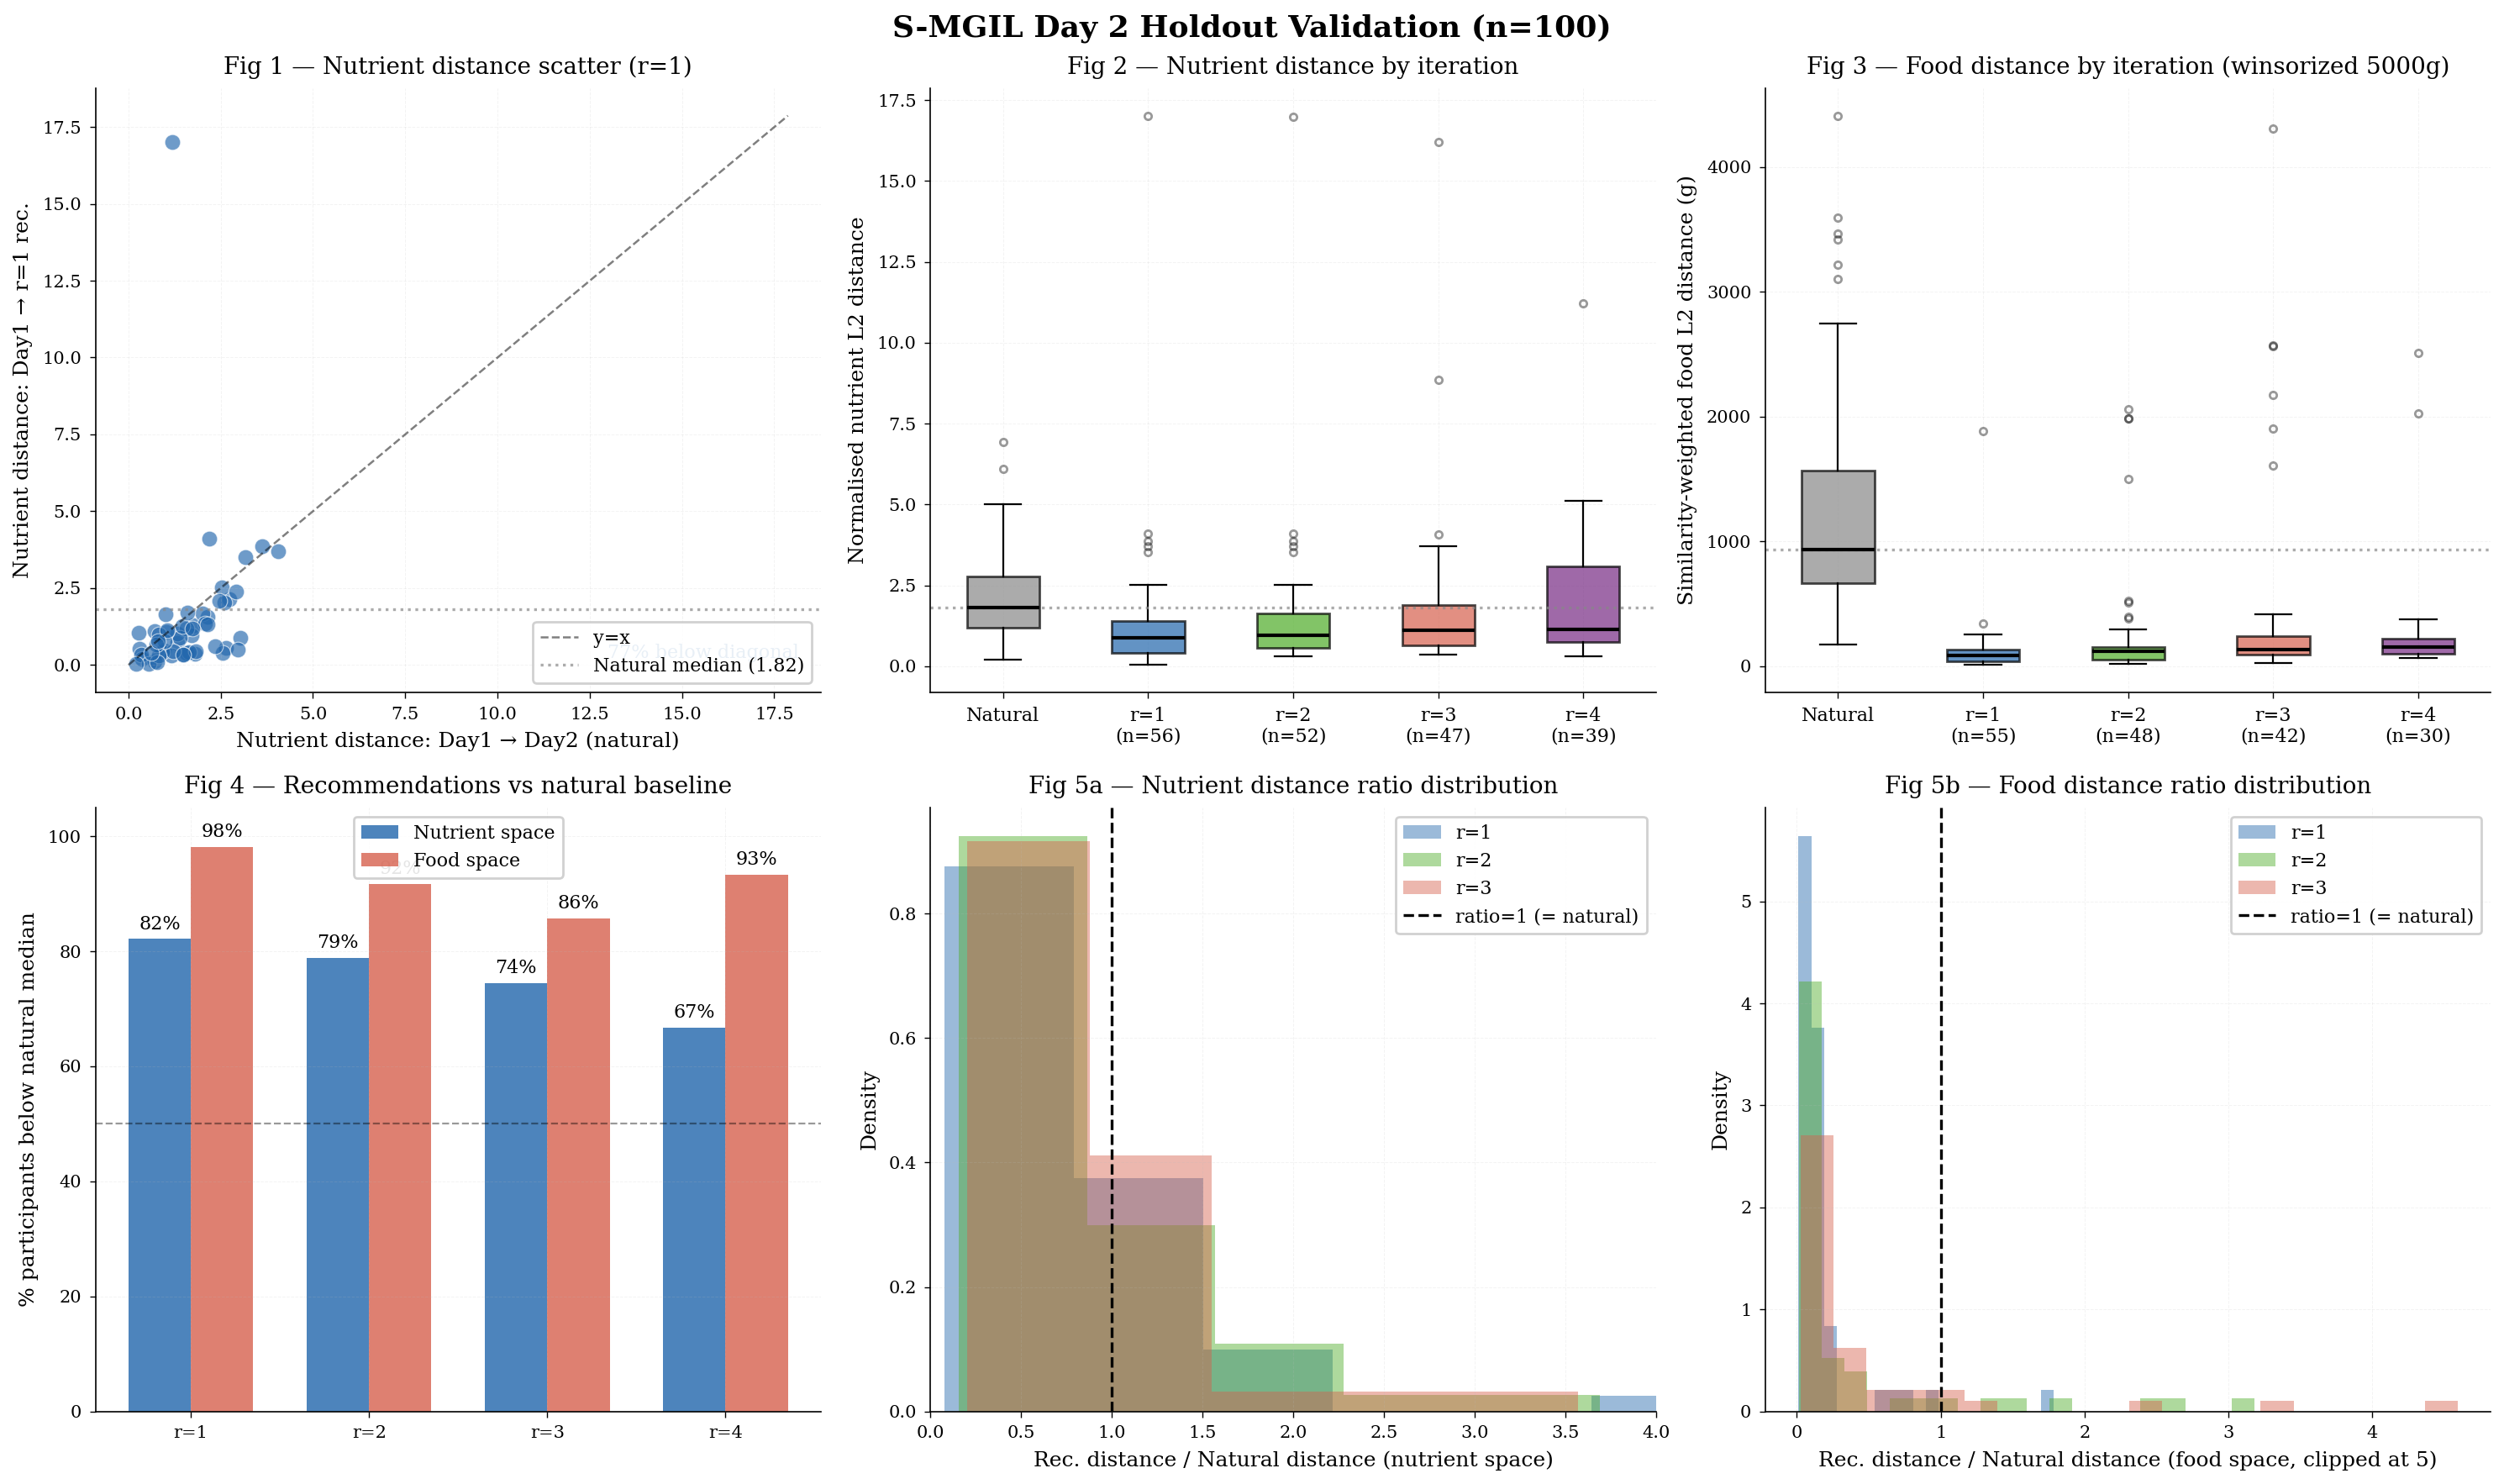
\includegraphics[width=\columnwidth]{smgil_validation_figures.png}
\caption{NHANES Day~2 holdout validation results ($n{=}345$ amenable
participants at $r{=}1$). \textbf{Fig.~1}: Nutrient distance scatter
($r{=}1$ vs.\ natural); 74\% of points fall below the diagonal,
indicating recommendations closer to Day~1 than the participant's own
Day~2 diet (dotted line: cohort natural median, 3.14). \textbf{Fig.~2}:
Normalised nutrient L2 distance by iteration (dotted line: natural
median). \textbf{Fig.~3}: Similarity-weighted food L2 distance by
iteration, winsorized at 5,000~g (dotted line: natural median).
\textbf{Fig.~4}: Percentage of participants below the natural median by
iteration and metric (nutrient: blue; food: red). \textbf{Figs.~5a--5b}:
Recommendation-to-natural distance ratio distributions at $r{=}1,2,3$;
mass left of the dashed line ($\text{ratio}{=}1$) indicates
recommendations within natural variation.}
\label{fig:nhanes_validation}
\end{figure}

\subsection{MyFitnessPal Results}
\label{subsec:mfp_results}

\subsubsection{Cohort Characteristics}

In contrast to NHANES, all 200 MFP users received at least one SGIO
recommendation (0\% non-amenable rate). This striking difference reflects
the broader dietary repertoire captured across multi-day food logs: the
larger augmented item space ($|\Faug| \approx 1{,}700$ vs.\ 135 in
NHANES) provides the optimizer with sufficient substitution flexibility
to satisfy DASH constraints for all users within the behavioral cost
budget. Median cohort characteristics: 28 logged days (training
period), 1,724~kcal/day, and 9 distinct foods per day.

\subsubsection{Nutrient-Space Results}

Table~\ref{tab:mfp_results} reports results for the MFP cohort.
Fig.~\ref{fig:mfp_validation} provides visual summaries.

SGIO recommendations at $r{=}1$ achieve a median normalized nutrient
distance of 1.637 from the training-period mean, compared to a natural
train-to-test median of 3.092 --- a 47\% reduction (Wilcoxon $W{=}153$,
$p{<}0.001$). In food-item space, 95\% of $r{=}1$ recommendations fall
below the individual's natural test-period distance, and 92\% fall below
the cohort natural median across both metric spaces.

The marginal cost of satisfying additional DASH constraints is negligible
across iterations ($\Delta D^{\bW}_{r=1 \to r=4} \approx 0$), indicating
that MFP users can achieve compliance with multiple DASH targets at
essentially no additional behavioral burden beyond the first-iteration recommendation.
Accordingly, running a single constraint-activation step ($r{=}1$) is
sufficient for this data modality --- all ten DASH constraints are
already satisfied in the $r{=}1$ solution, and further iterations add
no meaningful behavioral burden. This behavior contrasts with NHANES, where each iteration
incurs a meaningful marginal cost, and arises structurally from the
larger item space: with $|\Faug| \approx 1{,}700$ candidate foods, the
optimizer finds DASH-compliant substitutions among similar items at
near-zero switching cost.

\begin{table}[t]
\caption{SGIO MyFitnessPal Temporal-Split Validation Results ($N{=}200$)}
\label{tab:mfp_results}
\begin{center}
\begin{tabular}{lcccc}
\toprule
 & \multicolumn{2}{c}{\textbf{Nutrient Distance}}
 & \multicolumn{2}{c}{\textbf{Food Distance (srv)}} \\
\cmidrule(lr){2-3}\cmidrule(lr){4-5}
 & Median & \%\,below$^{\dagger}$ & Median & \%\,below$^{\dagger}$ \\
\midrule
Natural (train$\to$test) & 3.092 & --- & 1.195 & --- \\
\midrule
$r{=}1$ ($n{=}200$) & 1.637 & 92\% & 0.643 & 91\% \\
\bottomrule
\multicolumn{5}{l}{%
  \footnotesize $^{\dagger}$\% users below cohort natural median.}\\
\multicolumn{5}{l}{%
  \footnotesize All recommendation distances significant ($p{<}0.001$,}\\
\multicolumn{5}{l}{%
  \footnotesize one-sided Wilcoxon signed-rank test).}\\
\multicolumn{5}{l}{%
  \footnotesize Marginal costs across $r{=}1$--$4$ negligible
  ($\Delta D^{\bW}{<}0.01$);}\\
\multicolumn{5}{l}{%
  \footnotesize $r{=}1$ is the recommended activation step for this modality.}
\end{tabular}
\end{center}
\end{table}

\begin{figure}[t]
\centering
%% PLACEHOLDER: smgil_mfp_validation_final.png
%% 6-panel figure (a)--(f): scatter (r=1 vs natural), nutrient distance
%% boxplots, food distance boxplots, nutrient ratio dist., food ratio dist.,
%% fraction below natural median
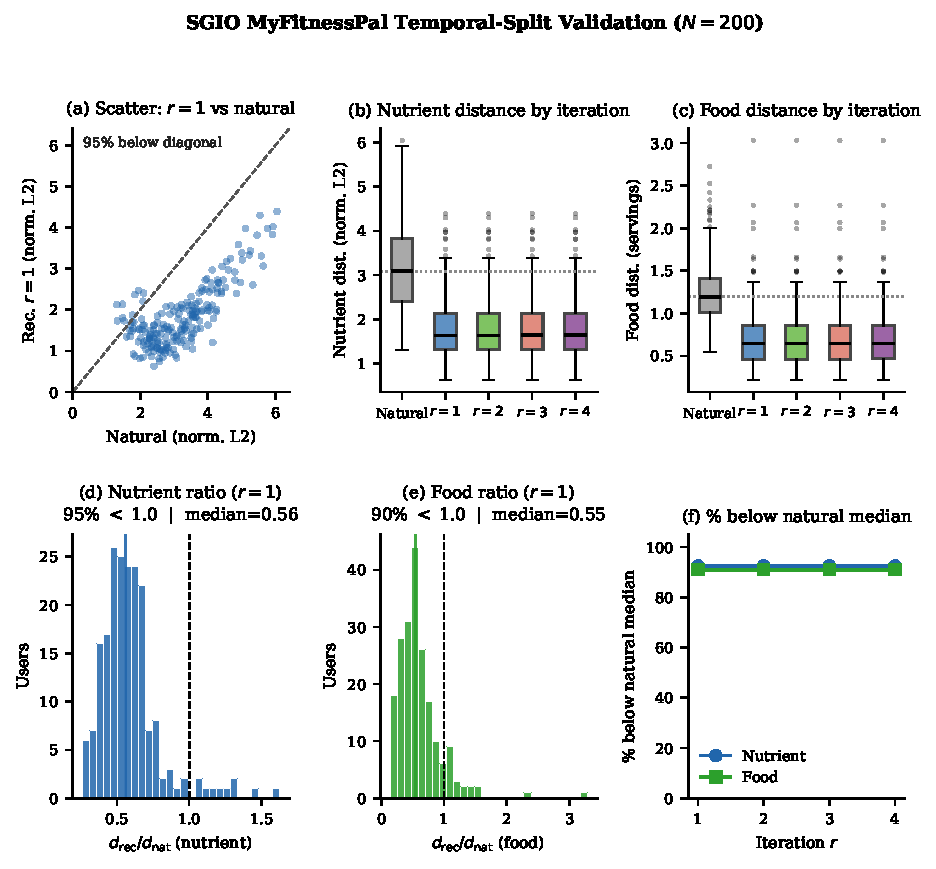
\includegraphics[width=\columnwidth]{smgil_mfp_validation_final.pdf}
\caption{MFP temporal-split holdout validation results ($N{=}200$,
0\% non-amenable). \textbf{Panel~(a)}: Nutrient distance scatter
($r{=}1$ vs.\ natural); 95\% of points fall below the diagonal.
\textbf{Panels~(b)--(c)}: Nutrient and food-space distances by iteration
(dotted line: natural median). \textbf{Panels~(d)--(e)}: Ratio
distributions $d_{\mathrm{rec}}/d_{\mathrm{nat}}$ at $r{=}1$; 95\%
and 90\% of users fall below 1.0 in nutrient and food space respectively.
\textbf{Panel~(f)}: Fraction of users below the natural median by
iteration.}
\label{fig:mfp_validation}
\end{figure}

%% ============================================================
\section{Discussion}
\label{sec:discussion}
%% ============================================================

\textbf{DASH-feasible recommendations within natural behavioral range.}
SGIO recommendations are fully DASH-feasible by construction: the
primal feasibility constraint $Az \leq b$ is enforced at every
iteration, so any $z_\ell$ satisfies all ten DASH nutrient bounds
simultaneously. The tradeoff path controls \emph{constraint activation},
not compliance level: at $r{=}4$ four constraints are actively binding,
and the behavioral cost increases monotonically. Even at $r{=}4$, this
cost remains within natural day-to-day dietary variation ($p{<}0.001$
in both nutrient and food-item space across $n{=}345$ amenable
participants). Put differently, the revised diet, constrained to meet
four DASH nutrient targets, remained close to each participant's
habitual diet. Only 11 of 356 (3\%) were non-amenable, confirming broad
applicability; the threshold $\tau$ is tunable for more or less
conservative deployment. Non-amenable participants are better served by
dietitian-led interventions than by algorithmic swapping.

\textbf{Data modality shapes recommendation feasibility.}
The contrast between NHANES (3\% non-amenable, meaningful marginal costs)
and MFP (0\% non-amenable, negligible marginal costs) reflects three
structural differences: NHANES captures a single 24-hour recall that
may represent an atypically extreme day, while MFP averages many logged
days; the MFP augmented item space ($|\Faug| \approx 1{,}700$ vs.\
135) makes low-cost substitution paths far more likely; and MFP attracts
self-selected, motivated food loggers who already eat closer to DASH
targets on average. On MFP, the flat marginal cost ($\Delta D^{\bW}
\approx 0$) collapses the tradeoff path to a single clinically actionable
step. MFP micronutrient data are substantially weaker than macronutrient
data---sodium correlation $\rho{=}0.53$, cholesterol
$\rho{=}0.51$~\cite{evenepoel2020mfp,morello2025mfp}---so MFP
results should be read as demonstrating \emph{algorithmic
generalizability} to a multi-day food log modality, not as a rigorous
epidemiological assessment of DASH compliance.

\textbf{Limitations and future directions.}
Several limitations warrant acknowledgment. First, SGIO operates on a
flat daily item-quantity vector: a nutritionally valid swap may lack
meal-level coherence (e.g., Greek yogurt replacing mayonnaise on a
sandwich) or may implicitly assume serving volumes that differ from
typical consumption. Second, both NHANES and MFP capture restaurant and
takeaway meals where individual swaps are not under the consumer's
control; a practical near-term scope restriction is to focus
recommendations on home-prepared meals, where ingredient choices are
directly actionable. Third, the current constraint set includes total
fat as a hard bound; evidence from dietary trials suggests that
foregrounding the nutrients most critical for blood pressure---sodium
reduction, potassium, and fiber---would better align the constraint set
with the DASH diet's primary cardiovascular mechanism. Fourth, the
similarity matrix encodes population-average substitutability and does
not capture individual constraints such as allergies, cultural
restrictions, or taste preferences. Fifth, personalization is currently
item-level: two participants with identical Day~1 records receive
identical recommendations regardless of dietary history. The
multi-observation formulation (Section~\ref{subsec:multi_obs}) begins
to address this by recovering constraints that are consistently binding
across multiple days; applying it to datasets with complete weighed food
records---such as those available from prior DASH feeding
studies---is a high-priority next step. Future work should also add an
LP comparison baseline and a component ablation of the similarity
architecture to quantify what preference recovery and the LLM reranker
each contribute.

\textbf{Prospective validation.}
These results provide preliminary evidence in support of the SGIO
framework to facilitate healthy eating concordant with the DASH dietary
pattern. Prospective validation linking recommendations to observed
dietary change and clinical outcomes---most directly, blood pressure
reduction---is the essential next step for clinical translation.

%% ============================================================
\section{Conclusion}
\label{sec:conclusion}
%% ============================================================

We proposed SGIO, a framework integrating food item similarity into the
inverse learning optimization backbone to produce personalized,
item-level dietary swap recommendations. By expanding each participant's
observed item space with high-similarity neighbors and encoding
substitutability as switching costs in the MGIL objective, SGIO
simultaneously satisfies DASH nutritional constraints, minimizes
behavioral disruption, and generates human-interpretable food swap
sequences. The multi-observation extension provides a principled
treatment of longitudinal dietary data that captures consistently binding
nutritional limits. All key theoretical guarantees of the underlying MGIL
framework (monotone tradeoff, nested face structure, forward optimality,
and $K$-independence) are preserved under both formulations.

Holdout validation across two dietary data modalities demonstrates that
the SGIO framework generalizes across data collection mechanisms. On the
primary NHANES cohort ($n{=}356$), recommendations fall within natural
intra-person dietary variation through \emph{all four}
constraint-tightening iterations ($p{<}0.001$ at every $r \in \{1,2,3,4\}$
in both nutrient and food-item spaces), with 76--80\% of participants
below the cohort natural nutrient-distance median and 81--84\% below the
natural food-distance median. The uniformly significant result across
iterations indicates that SGIO recommendations are behaviorally feasible
even at maximum DASH constraint satisfaction for this cohort. The 3\%
non-amenable rate demonstrates broad applicability, with only a small
minority requiring alternative clinical intervention pathways.

On the MFP cohort ($n{=}200$), SGIO achieves a 47\% median nutrient
distance reduction ($W{=}153$, $p{<}0.001$) with a 0\% non-amenable
rate, demonstrating that multi-day food logs provide sufficient dietary
context for universal recommendation coverage. The contrast between the
low NHANES non-amenable rate (3\%) and the MFP rate (0\%), alongside the
structural difference in item-space size ($|\Faug| \approx 135$ vs.\
$1{,}700$), provides a quantitative characterization of how data
collection modality shapes recommendation feasibility. Together, these
results establish SGIO as a behaviorally grounded, optimization-principled
framework for precision dietary counseling, with deployment
characteristics that adapt systematically to the dietary data source.

%% ============================================================
\begin{thebibliography}{00}

\bibitem{ahmadi2024IL}
F. Ahmadi, F. Ganjkhanloo, and K. Ghobadi,
``From non-identifiability to goal-integrated decision-making in
parametric inverse optimization,''
\textit{arXiv preprint arXiv:2603.17033}, 2026.
[Online]. Available: \url{https://doi.org/10.48550/arXiv.2603.17033}

\bibitem{sacks2001effects}
F. M. Sacks et al.,
``Effects on blood pressure of reduced dietary sodium and the dietary
approaches to stop hypertension (DASH) diet,''
\textit{New England Journal of Medicine}, vol.~344, no.~1,
pp.~3--10, 2001.

\bibitem{liese2009adherence}
A. D. Liese et al.,
``Adherence to the DASH diet is inversely associated with incidence
of type 2 diabetes: The insulin resistance atherosclerosis study,''
\textit{Diabetes Care}, vol.~32, no.~8, pp.~1434--1436, 2009.

\bibitem{CDC_2020}
Centers for Disease Control and Prevention,
``National Health and Nutrition Examination Survey (NHANES),
2017--2018,'' U.S. Dept.\ of Health and Human Services, 2020.
[Online]. Available: \url{https://www.cdc.gov/nchs/nhanes/}

\bibitem{usda_2019}
U.S. Department of Agriculture,
``USDA FoodData Central,'' 2019.
[Online]. Available: \url{https://fdc.nal.usda.gov/}

\bibitem{beaton1979sources}
G. H. Beaton et al.,
``Sources of variance in 24-hour dietary recall data: Implications
for nutrition study design and interpretation,''
\textit{American Journal of Clinical Nutrition}, vol.~32, no.~12,
pp.~2546--2559, 1979.

\bibitem{besbes2023contextual}
O. Besbes, Y. Fonseca, and I. Lobel,
``Contextual inverse optimization: Offline and online learning,''
\textit{Operations Research}, vol.~71, no.~4, pp.~1105--1123, 2023.

\bibitem{aswani2018inverse}
A. Aswani, Z. Shen, and A. Siddiq,
``Inverse optimization with noisy data,''
\textit{Operations Research}, vol.~66, no.~3, pp.~870--892, 2018.

\bibitem{chan2014generalized}
T. C. Y. Chan, T. Lee, and D. Terekhov,
``Generalized inverse multiobjective optimization with application
to cancer therapy,''
\textit{Operations Research}, vol.~62, no.~3, pp.~680--695, 2014.

\bibitem{elmachtoub2022smart}
A. N. Elmachtoub and P. Grigas,
``Smart ``predict, then optimize'',''
\textit{Management Science}, vol.~68, no.~1, pp.~9--26, 2022.

\bibitem{lin2024conformal}
Y. Lin and M. Ghassemi,
``Conformal inverse optimization,''
\textit{arXiv preprint arXiv:2402.01489}, 2024.

\bibitem{zattoni2025learning}
A. Zattoni Scroccaro, B. Amos, P. Mohajerin Esfahani, and
S. Kamalaruban,
``Learning in inverse optimization: Incenter cost,
augmented suboptimality loss, and algorithms,''
\textit{Operations Research}, 2025.

\bibitem{mfp_kaggle}
Z. Kiknozadze,
``MyFitnessPal food diary dataset,'' Kaggle, 2020.
[Online]. Available:
\url{https://www.kaggle.com/datasets/zvikinozadze/myfitnesspal-dataset}

\bibitem{johnson2019faiss}
J. Johnson, M. Douze, and H. J\'{e}gou,
``Billion-scale similarity search with GPUs,''
\textit{IEEE Transactions on Big Data}, vol.~7, no.~3,
pp.~535--547, 2021.

\bibitem{zhang2025qwen3embedding}
P. Zhang et al.,
``Qwen3-Embedding: Advancing text embedding and reranking through
foundation models,''
\textit{arXiv preprint arXiv:2506.05176}, 2025.

\bibitem{evenepoel2020mfp}
C. Evenepoel, E. Clevers, L. Deroover, W. Van Loo, C. Matthys, and K. Verbeke,
``Accuracy of nutrient calculations using the consumer-focused online
app MyFitnessPal: Validation study,''
\textit{J. Med. Internet Res.}, vol.~22, no.~10, p.~e18237, Oct. 2020.
doi: 10.2196/18237.

\bibitem{morello2025mfp}
O. Morello, L. McPhee, M. Kucab, N. Bellissimo, and J. O. Totosy de Zepetnek,
``Reliability and validity of nutrient assessment applications for
Canadian endurance athletes: MyFitnessPal and Cronometer,''
\textit{J. Hum. Nutr. Diet.}, vol.~38, pp.~1--16, 2025.
doi: 10.1111/jhn.70148.

\bibitem{jones2025aha}
D. W. Jones et al.,
``2025 AHA/ACC/AANP/AAPA/ABC/ACCP/ACPM/AGS/AMA/ASPC/NMA/PCNA/SGIM
Guideline for the Prevention, Detection, Evaluation, and Management of
High Blood Pressure in Adults,''
\textit{Circulation}, vol.~152, no.~11, pp.~e1--e222, 2025.
doi: 10.1161/CIR.0000000000001356.

\bibitem{appel1997dash}
L. J. Appel et al.,
``A clinical trial of the effects of dietary patterns on blood pressure,''
\textit{New England Journal of Medicine}, vol.~336, pp.~1117--1124, 1997.

\bibitem{appel2003premier}
L. J. Appel et al.\ (Writing Group of the PREMIER Collaborative Research Group),
``Effects of comprehensive lifestyle modification on blood pressure control:
main results of the PREMIER clinical trial,''
\textit{JAMA}, vol.~289, no.~16, pp.~2083--2093, 2003.

\bibitem{blumenthal2010premier}
J. A. Blumenthal et al.,
``Effects of the DASH diet alone and in combination with exercise and weight
loss on blood pressure and cardiovascular biomarkers in men and women with
high blood pressure,''
\textit{Archives of Internal Medicine}, vol.~170, no.~2, pp.~126--135, 2010.
doi: 10.1001/archinternmed.2009.470.

\end{thebibliography}

\end{document}